\documentclass [12pt]{article}
\setlength{\textwidth}{6.25in}
\setlength{\textheight}{8.5in}
\setlength{\evensidemargin}{0in}
\setlength{\oddsidemargin}{0in}
\setlength{\topmargin}{-0.1in}
\setlength{\parskip}{.1in}  
\setlength{\parindent}{0.0in}  
\usepackage[left=3.5cm,right=2.5cm]{geometry}


\setcounter{secnumdepth}{4}
\setcounter{tocdepth}{4}
   
\usepackage{amsmath}
\usepackage{amssymb}
\usepackage{enumitem}
\numberwithin{equation}{section}
%\renewcommand{\theequation}{\thesection\arabic{equation}}

%NOTES

\usepackage{xargs}                      % Use more than one optional parameter in a new commands
\usepackage[pdftex,dvipsnames]{xcolor}  % Coloured text etc.
% 
\usepackage[colorinlistoftodos,prependcaption,textsize=tiny]{todonotes}
\newcommandx{\unsure}[2][1=]{\todo[linecolor=red,backgroundcolor=red!25,bordercolor=red,#1]{#2}}
\newcommandx{\change}[2][1=]{\todo[linecolor=blue,backgroundcolor=blue!25,bordercolor=blue,#1]{#2}}
\newcommandx{\info}[2][1=]{\todo[linecolor=OliveGreen,backgroundcolor=OliveGreen!25,bordercolor=OliveGreen,#1]{#2}}
\newcommandx{\improvement}[2][1=]{\todo[linecolor=Plum,backgroundcolor=Plum!25,bordercolor=Plum,#1]{#2}}
\newcommandx{\thiswillnotshow}[2][1=]{\todo[disable,#1]{#2}}




\definecolor{gold(metallic)}{rgb}{0.83, 0.69, 0.22}

\newcommand{\hwplotR}{\raisebox{2pt}{\tikz{\draw[red,solid,line width=0.9pt](0,0) -- (5mm,0);}}}
\newcommand{\hwplotY}{\raisebox{2pt}{\tikz{\draw[gold(metallic),solid,line width=0.9pt](0,0) -- (5mm,0);}}}
\newcommand{\hwplotG}{\raisebox{2pt}{\tikz{\draw[green,solid,line width=0.9pt](0,0) -- (5mm,0);}}}
\newcommand{\hwplotB}{\raisebox{2pt}{\tikz{\draw[blue,solid,line width=0.9pt](0,0) -- (5mm,0);}}}
\newcommand{\hwplotK}{\raisebox{2pt}{\tikz{\draw[black,dashed,line width=1.2pt](0,0) -- (5mm,0);}}}
\newcommand{\hwplotT}{\raisebox{2pt}{\tikz{\draw[black,solid,line width=1.2pt](0,0) -- (5mm,0);}}}


\usepackage{graphicx} % Used to insert images
\usepackage{adjustbox} % Used to constrain images to a maximum size 

\usepackage{bm}
%\usepackage[textsize=scriptsize]{todonotes}
\usepackage[hypcap]{caption}

\usepackage[hidelinks]{hyperref}




\usepackage{amsthm}
\newtheorem{prop}{Proposition}




%\usepackage{fontspec}
%\setmainfont{Times New Roman}
\setlength{\parskip}{.1in}  
\setlength{\parindent}{0.0in}  
\renewcommand{\baselinestretch}{1.5}
\renewcommand\contentsname{Contenido}
\renewcommand{\figurename}{Fig.}
\renewcommand{\listfigurename}{Lista de Figuras}
\usepackage{tikz}
%\usetikzlibrary{arrows,shapes,trees,..}
%\usepackage{pgflibraryarrows}
%\usepackage{pgflibrarysnakes}

\usepackage{longtable}
\usepackage[nottoc,numbib]{tocbibind}
\usepackage[round,sort]{natbib}
\renewcommand\refname{Referencias}

\newcommand{\myparagraph}[1]{\paragraph{#1}\mbox{}\\}
\newcommand{\PP}{\textit{\tiny P}}
\newcommand{\C}{\textit{\tiny C}}
\newcommand{\R}{\textit{\tiny R}}
\newcommand{\CR}{\textit{\tiny CR}}
\newcommand{\PC}{\textit{\tiny PC}}
\newcommand{\PR}{\textit{\tiny PR}}
\newcommand{\CP}{\textit{\tiny CP}}
\newcommand{\RC}{\textit{\tiny RC}}
\newcommand{\RP}{\textit{\tiny RP}}


%AMSMATH environment

\makeatletter
\newcommand{\mathleft}{\@fleqntrue}
\newcommand{\mathcenter}{\@fleqnfalse}
\makeatother

%Tikz===========================================

\usepackage{tikz,pgfplots}
\usetikzlibrary{arrows,calc}
\newenvironment{customlegend}[1][]{%
    \begingroup
    % inits/clears the lists (which might be populated from previous
    % axes):
    \csname pgfplots@init@cleared@structures\endcsname
    \pgfplotsset{#1}%
}{%
    % draws the legend:
    \csname pgfplots@createlegend\endcsname
    \endgroup
}%

% makes \addlegendimage available (typically only available within an
% axis environment):
\def\addlegendimage{\csname pgfplots@addlegendimage\endcsname}

%%--------------------------------

% definition to insert numbers
\pgfkeys{/pgfplots/number in legend/.style={%
        /pgfplots/legend image code/.code={%
            \node at (0.295,-0.0225){#1};
        },%
    },
}
%%===================================

\begin{document}

\subsection{Influencia de $k_{ij}$ sobre $f$}

Sin importar la estrategia de forrajeo tenemos que :
\begin{enumerate}[label=(\alph*)]
\item \begin{equation}
  \lim_{k_{ij} \to  0 }f(k_{ij}) = \lim_{k_{ij} \to 0 }\frac{g(k_{ij}) a}{1+k_{ij}^\phi} = 0 
\end{equation}
ya que $ g(k_{ij}) \to (k_{ij} \to 0)$ y $\frac{a}{1+k_{ij}^\phi} < a$  para todo $k_{ij}$
\item 
\begin{equation}
\lim_{k_{ij} \to  0 }f(k_{ij}) - ag(k_{ij}) = 0
\end{equation}
y por lo tanto $f \approx a g(k_{ij})$ para $k_{ij}$ suficientemente peque\~no , donde $g(k_{ij}) = f(k_{ij})\Pi(k_{ij})$.
\item $f_{3D} > f_{2D} \iff k_{ij} > 1$ donde $f_{nD}$ representa al valor de $f$ para espacios de b\'usqueda \emph{n-dimensionales}
\end{enumerate}

A continuaci\'on se analizan propiedades de $f$ que a nivel \emph{cuantitativo} difieren entre las distintas estrategias de forrajeo

\subsubsection{Grazing}

\begin{prop}
  $f$ tiene un punto m\'aximo en $\mathbb{R}^+$ si y solo s\'i $\phi > (D_i - 1)p_d$ 
\end{prop}

\begin{proof}
\mbox{}\\
Sea $ h = (D_i-1)p_d$\\
Dado que $f$ es diferenciable y:
  \begin{equation}
    \begin{aligned}
      f'(k_{ij}) &= a \frac{h k_{ij}^{h-1} (1 + k_{ij}^\phi) -\phi k_{ij}^{\phi-1+h}}{(1+k_{ij}^{\phi})^2} \\
            &= a \frac{(h-\phi)k_{ij}^{h-1 + \phi}  + h k_{ij}^{h-1} }{(1+k_{ij}^{\phi})^2}\\
            &= a \frac{(h-\phi)k_{ij}^\phi + h }{(1+k_{ij}^{\phi})^2}\\
     \end{aligned}
  \end{equation}
Luego tenemos que $f'$ posee un \emph{cero} en $\mathbb{R}^+$ si y solo s\'i $ h< \phi$ y en caso afirmativo tenemos que $k^*$ tal que $f(k^*) = 0$ es $(\frac{h}{\phi-h})^{\frac{1}{\phi}}$ adem\'as:
\begin{equation}
  f'(x) :
  \begin{cases}
    < 0 &; k_{ij}  > k^* \\
    > 0 &; k_{ji} < k^*
  \end{cases}
\end{equation}

Lo que indica que $k^*$ es un punto m\'aximo.
\end{proof}

De la proposici\'on anterior tambi\'en vemos la dependencia de $k^*$ en $\phi$, teniendo $h$ fijo en nuestro caso se observa que si $\phi$ esta suficientemente cercano a $h$ , $k^*$ es extremadamente grande, sin embargo se observa un decaim\'iento muy r\'apido y para valores de $\phi \geq 2h$  , $k^*$ se encuentra pr\'oximo a 1(y en realidad converge a 1 para $\phi \to \infty$) , v\'ease figura \ref{fig:kmaxGrazing}. \\

\begin{figure}
\begin{center}
 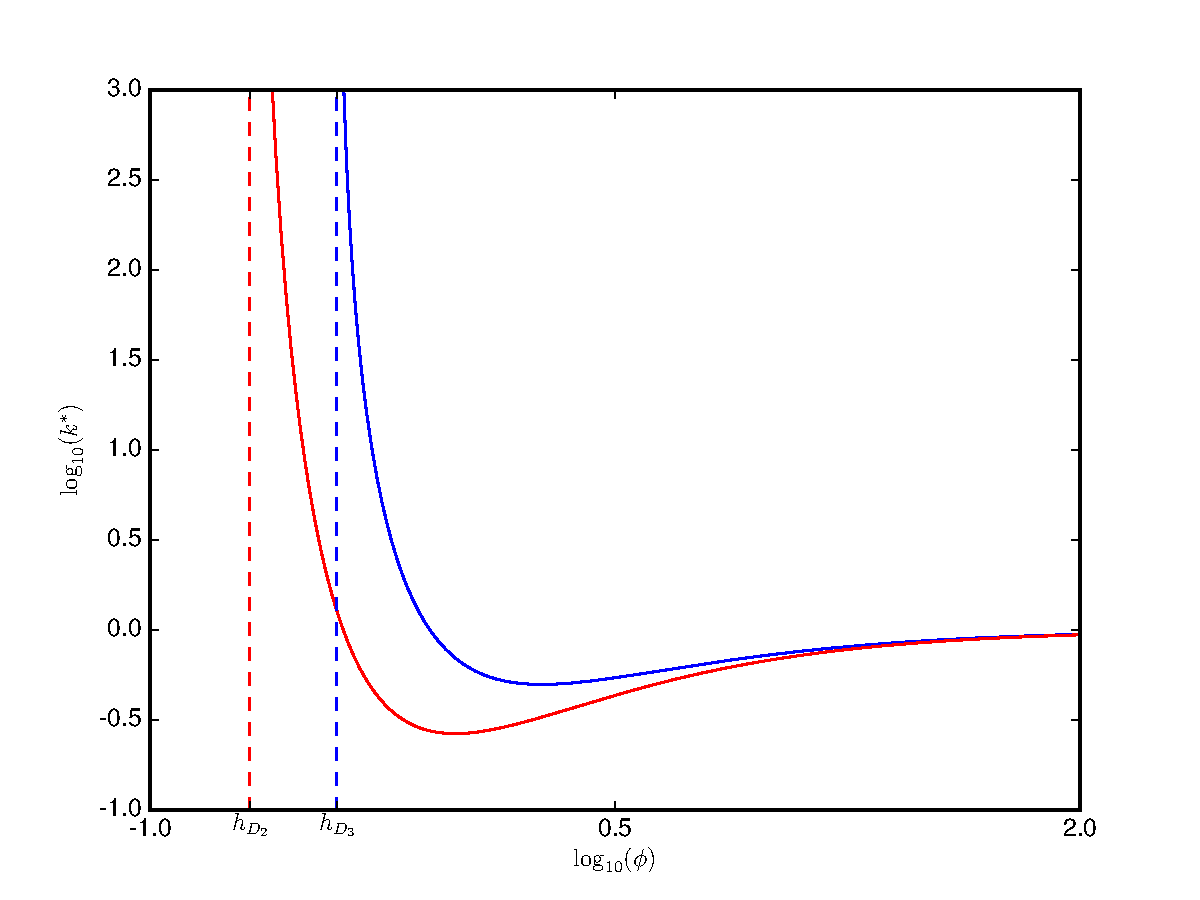
\includegraphics[width=0.9\textwidth]{./Plots/kmaxGrazing.pdf}
 \caption[$k^*, Grazing$]{$k^*$ en funci\'on a $\phi$ donde se observa la divergencia para valores cercanos a $h$ y la convergencia a 1 para valores elevados de $\phi$, ({\hwplotB}) es para el caso de ambientes de b\'usqueda $3D$ y ({\hwplotR}) $2D$, $h_{3D}$ y $h_{2D}$ denotan los l\'imites inferiores para $\phi$ que permiten la existencia de $k^*$}
 \label{fig:kmaxGrazing} 
\end{center}
\end{figure}



En el caso que $\phi < h$ tenemos que $f$ es mon\'otona creciente. Ambos casos se grafican en la figura \ref{fig:f1Grazing}.

\begin{figure}
\begin{center}
 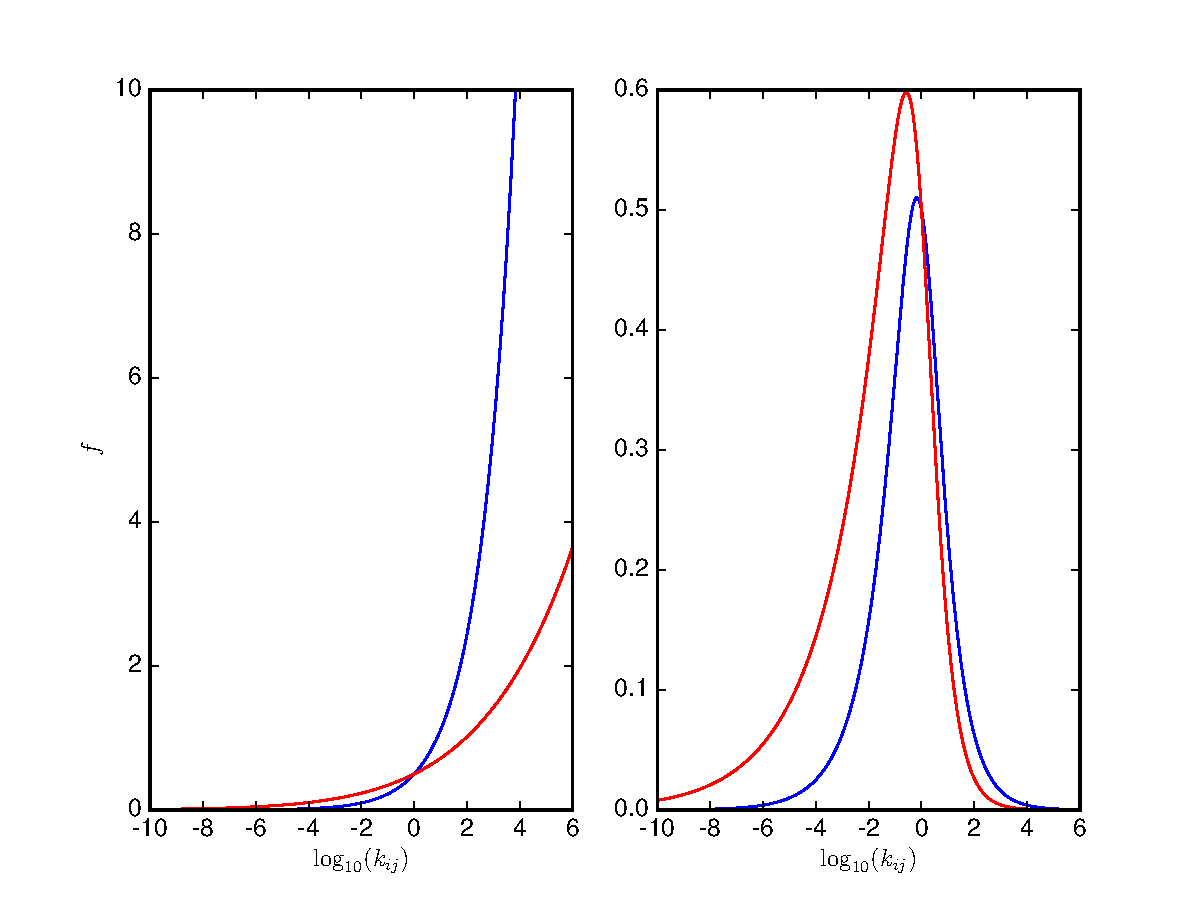
\includegraphics[width=0.9\textwidth]{./Plots/f1Grazing.pdf}
 \caption[$f_1, Grazing$]{$f$ en funci\'on a $k_{ij}$, con $a =1$, en el panel de la izquierda tenemos $b = 0.1$ y en el de la derecha $b=1.$ , ({\hwplotB}) es para el caso de ambientes de b\'usqueda $3D$ y ({\hwplotR}) $2D$}
 \label{fig:f1Grazing} 
\end{center}
\end{figure}


\subsubsection{Sit}

Se tiene cualitativamente las m\'ismas caracter\'isticas que en el caso anterior, con la diferencia que en este caso $ h:= p_v + 2(D_i -1) p_d$, y por ende para $\phi \in ]2(D_i - 1) p_d , p_V + 2(D_i -1)p_d[$ tendr\'iamos un comportamiento mon\'ontono para $f_{sit}$ y la existencia de un m\'aximo para $f_{grazing}$.\\

La figura \ref{fig:f1Sit} muestra las semejanzas con el caso anterior, salvo la diferencia que en este caso $k^*>1$ para el caso $3D$ y adem\'as alcanza un valor m\'as alto que el caso $2D$.\\
En general tenemos que $ k^*_{Sit} > k^*_{grazing}$ .

\begin{figure}
\begin{center}
 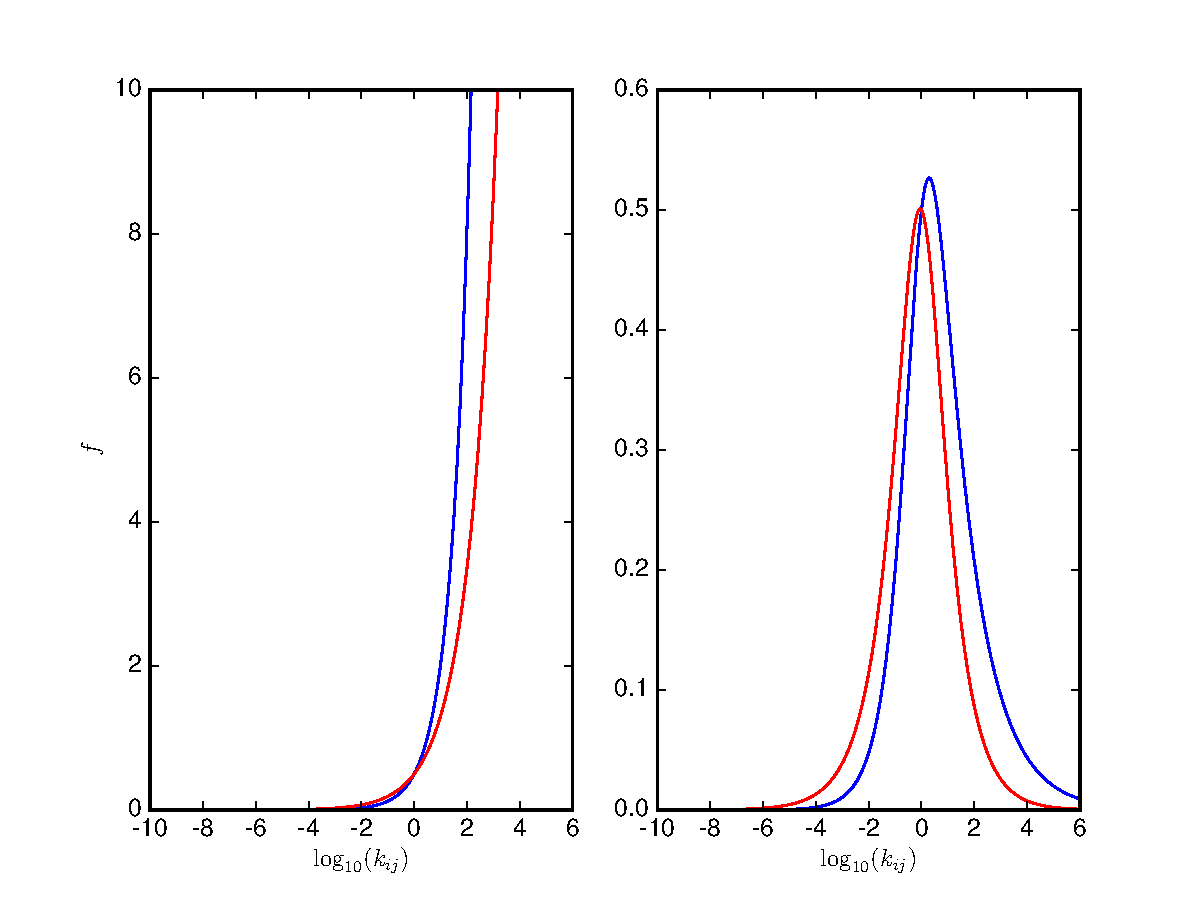
\includegraphics[width=0.9\textwidth]{./Plots/f1Sit.pdf}
 \caption[$f_1, Sit$]{$f$ en funci\'on a $k_{ij}$, con $a =1$, para el caso de una estrategia de forrajeo \emph{Sit-and-Wait}, las dem\'as especificaciones se comparten con la figura \ref{fig:f1Grazing}}
 \label{fig:f1Sit} 
\end{center}
\end{figure}


\subsubsection{Captura activa}

En este caso tenemos un comportamiento similar al descrito previamente, esto es para $\phi > p_v + 2(D_i -1) p_d$ tenemos que $f$ decae exponencialmente a partir de un valor de $k_{ij}$ \emph{suficientemente grande}, y a su vez crece exponencialmente para valores \emph{suficientemente peque\~nos}, dado que $f \in C^1$ esto a su vez nos dice que debe existir un punto m\'aximo para $f$ sin embargo en este caso no tenemos una expresi\'on an\'alitica para $k^*$ salvo que cumple la siguiente relaci\'on:

\begin{equation}
  (k^*)^{\phi}((k^*)^{2p_v}(p_v+ h -\phi) + (h -\phi) + (k^*)^{2p_v - \phi}(p_v + h ) ) + h = 0
\end{equation}

Con $h$ igual que en el caso $grazing$.\\
De esta relaci\'on podemos obtener que :
\begin{equation}
  k^*_{Active} \in ] k^*_{Grazing} , k^*_{Sit} [
\end{equation}

A su vez para $\phi \leq 2(D_i - 1)p_d $ podemos esperar un crecimiento mon\'otono por parte de $f$. 

\begin{figure}
\begin{center}
 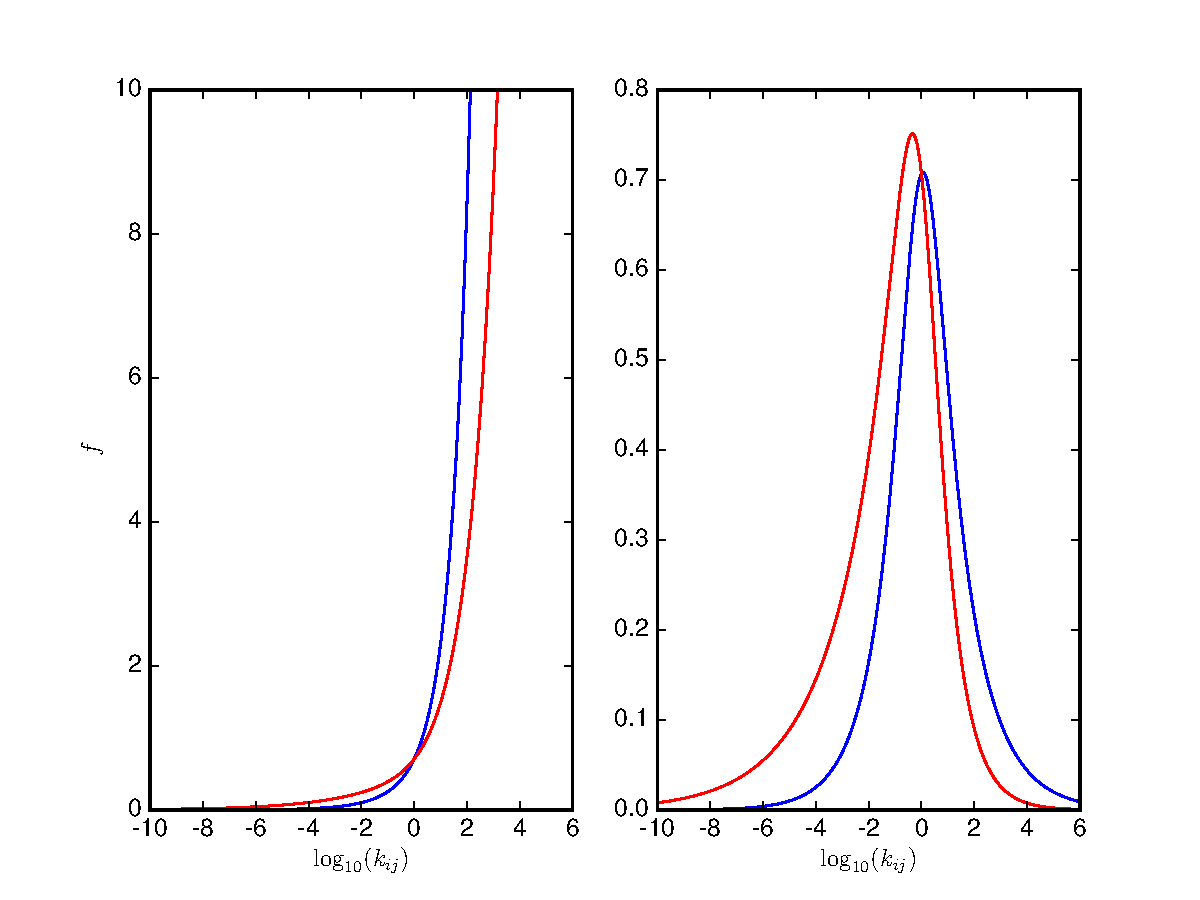
\includegraphics[width=0.9\textwidth]{./Plots/f1Active.pdf}
 \caption[$f_1, Active$]{$f$ en funci\'on a $k_{ij}$, con $a =1$, para el caso de una estrategia de forrajeo \emph{activa}, las dem\'as especificaciones se comparten con la figura \ref{fig:f1Grazing}}
 \label{fig:f1Active} 
\end{center}
\end{figure}




\end{document}
